% arara: lualatex: { shell: true }


\documentclass[
  tikz,
  convert={density=600,outext=.png},
]{standalone}

\usetikzlibrary{calc}
\usetikzlibrary{arrows.meta,automata,positioning}

\begin{document}

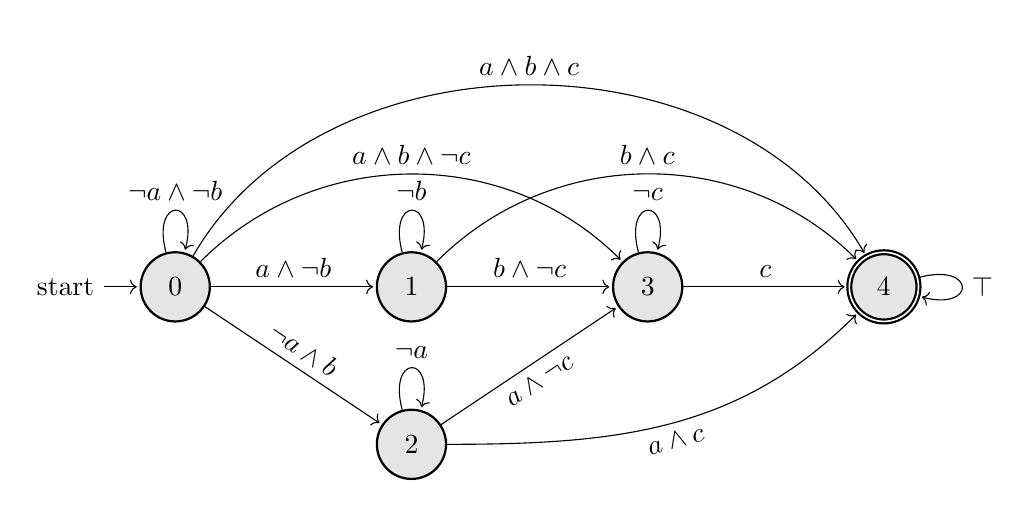
\begin{tikzpicture}[node distance=3cm,on grid,auto, shorten >=1pt]
	\tikzstyle{every state}=[fill={gray!20},thick]
	\tikzstyle{every node}=[transform shape]

	\node[initial,state] (q0) [] {$0$};
	\node[state] (q1) [right= of q0] {$1$};
	\node[state] (q2) [below=2cm of q1] {$2$};
	\node[state] (q3) [right= of q1] {$3$};
	\node[state,accepting] (qF) [right=of q3] {$4$};

	\path[->]
	% q0
	(q0) edge[loop above] node[] {$\neg a \land \neg b$} (q0)
	(q0) edge[] node[] {$a \land \neg b$} (q1)
	(q0) edge[] node[sloped] {$\neg a \land b$} (q2)
	(q0) edge[bend left=45] node[] {$a \land b \land \neg c$} (q3)
	(q0) edge[bend left=60] node[] {$a \land b \land c$} (qF)
	% q1
	(q1) edge[loop above] node[] {$\neg b$} (q1)
	(q1) edge[] node[] {$b \land \neg c$} (q3)
	(q1) edge[bend left=45] node[] {$b \land c$} (qF)
	% q2
	(q2) edge[loop above] node[] {$\neg a$} (q2)
	(q2) edge[] node[below,sloped] {$a \land \neg c$} (q3)
	(q2) edge[out=0,in=225] node[below,sloped] {$a \land c$} (qF)
	% q3
	(q3) edge[loop above] node[] {$\neg c$} (q3)
	(q3) edge[] node[] {$c$} (qF)
	% q4
	(qF) edge[loop right] node[] {$\top$} (qF)
	;
\end{tikzpicture}

\end{document}
